\chapter{Produit scalaire et orthogonalité} \label{chap:produit}
La notion de produit scalaire permet de définir la longueur, ou norme d'un vecteur, ainsi que l'orthogonalité de deux vecteurs.
Ces deux propriétés, norme et orthogonalité, permettent à leur tour de définir des bases dites orthonormées pour les espaces vectoriels.
L'utilisation de base orthonormées permet de simplifier énormément les calculs. En fait, lorsqu'on introduit les vecteur dans le plan $\BBR^2$ ou dans l'espace $\BBR^3$, on utilise tout naturellement des bases
orthonormées parce qu'elles constituent un choix naturel.

Dans ce chapitre, nous allons présenter le produit scalaire dans sa forme la plus générale et donner un simple aperçu
de la procédure pour obtenir une base orthonormée.  Bien que ceci puisse, en principe, permettre d'étudier
plusieurs applications intéressantes, nous devrons passer outre à leur étude faute de temps.
\section{Introduction}
\begin{defini}
Soit $V$ un espace vectoriel sur le corps $\BBR$. 
Pour chaque paire de vecteurs $\mat{u}, \mat{v}$ 
on peut associer un scalaire dénoté par 
$\langle\mat{u}, \mat{v}\rangle $,
qu'on désigne sous le nom de \Definition{produit scalaire} de ces deux vecteurs et 
satisfaisant les axiomes suivants:
\begin{enumerate}
\item $\langle a\mat{u} + b\mat{v}, \mat{w} \rangle = a \langle\mat{u}, \mat{w}\rangle + b\langle\mat{v}, \mat{w}\rangle $ pour 
$\mat{u}, \mat{v}, \mat{w} \in V$ et $a, b \in \BBR$.
\item$ \langle\mat{u}, \mat{v}\rangle = \langle\mat{v}, \mat{u}\rangle$
\item $\langle \mat{u}, \mat{u}\rangle \geq 0$
\item $\langle \mat{u}, \mat{u}\rangle = 0$ si et seulement si $\mat{u} = \zero$.
\end{enumerate}
\end{defini}

\begin{exerciceB}\label{ex:scalaire1}
Lorsqu'on a des nombres complexes, on ne peut pas définir un ordre, du plus grand au plus 
petit. \footnote{Pour donner un exemple concret, pour les réels on sait que $-1 < 0 < 1$; si 
on a le nombre complexe $i=\sqrt{-1}$, pouvez-vous décider si ce nombre est plus petit ou plus 
grand que zéro?} 
Sachant ceci, lorsqu'on définit un produit scalaire sur le corps
des complexes, expliquez comment la modification du deuxième axiome à

2. $ \langle\mat{u}, \mat{v}\rangle = \overline{\langle\mat{v}, \mat{u}\rangle}$

\noindent fait en sorte que le troisième axiome devienne possible.\footnote{Rappelons que
lorsqu'on met une barre au-dessus d'un nombre complexe, ceci indique que l'on prend son 
conjugué, remplaçant $i$ par $-i$.}
\end{exerciceB}

En utilisant le premier et le deuxième axiome, on peut vérifier que:
\[
\langle \mat{w}, a\mat{u} + b\mat{v} \rangle =  a \langle\mat{w}, \mat{u}\rangle 
+ b \langle\mat{w}, \mat{v}\rangle
\]

\begin{exerciceB}
Si on définit le produit scalaire sur le corps des complexes avec la modification mentionnée à
 l'\refexercice{ex:scalaire1}, démontrez que 
 \[
 \langle \mat{w}, a\mat{u} + b\mat{v} \rangle =  \bar{a} \langle\mat{w}, \mat{u}\rangle + \bar{b}\langle\mat{w}, \mat{v}\rangle
 \]
\end{exerciceB}

On définit également la \definition{norme} ou longueur d'un vecteur comme le nombre réel non négatif suivant:
\[
\norm{\mat{u}} = \sqrt{\langle\mat{u}, \mat{u} \rangle}
\]
À noter qu'en raison des propriétés de l'addition des vecteur, y compris le vecteur nul $\zero$, nous avons $\langle\mat{u} + \zero, \mat{v}\rangle = \langle\mat{u}, \mat{v}\rangle $; également, en utilisant le premier axiome de la définition ci-dessus, nous devons avoir
$\langle\mat{u} + \zero, \mat{v}\rangle = \langle\mat{u}, \mat{v}\rangle +  \langle\zero, \mat{v}\rangle$, d'où l'on tire 
$ \langle\zero, \mat{v}\rangle = \zero$.  De la même façon, on peut démontrer que $ \langle\mat{v}, \zero\rangle = \zero$
Nous pouvons maintenant prouver une importante propriété connue sous le nom 
d'\definition{inégalité de Cauchy-Schwarz}.
\begin{theo}
Soit $V$ un espace vectoriel sur le corps $\BBR$.
Pour tout vecteur $\mat{u}, \mat{v} \in V$ nous avons $ \abs{\langle\mat{u}, \mat{v}\rangle} \leq \norm{\mat{u}} \, \norm{\mat{v}}$.
Cette inégalité est connue sous le nom d'inégalité de Cauchy-Schwarz.
\proof 
On note que l'inégalité est satisfaite si $\mat{v}=\zero$. Nous allons maintenant considérer le cas $\mat{v}\neq\zero$
Définissons d'abord $z = \langle\mat{u}, \mat{v}\rangle$. 
Considérons ensuite l'inégalité
\[
0 \leq\norm{\mat{w}}^2 = \langle \mat{w}, \mat{w}\rangle
\]
avec le vecteur $\mat{w} = \mat{u} - \alpha z \mat{v}$ où $\alpha$ est un nombre réel que nous définirons plus tard.
Ceci nous donne:
\[
\begin{matrix}[rcl]
0 &\leq& \langle \mat{u} - \alpha z \mat{v},  \mat{u} - \alpha z \mat{v} \rangle \\
 &=& \langle \mat{u}, \mat{u} \rangle - \alpha z  \langle \mat{v}, \mat{u} \rangle - \alpha z \langle \mat{u}, \mat{v} \rangle + \alpha^2 z^2 
 \langle \mat{v}, \mat{v} \rangle \\
 &=& \norm{\mat{u}}^2 -2\alpha z^2 + \alpha^2 z^2   \norm{\mat{v}}^2
  \end{matrix}
\]
Choisissons maintenant $\displaystyle \alpha = \frac{1}{\norm{\mat{v}}^2}$; ceci nous donne
\[
0 \leq  \norm{\mat{u}}^2 - 2 \frac{z^2}{\norm{\mat{v}}^2} + \frac{z^2}{\norm{\mat{v}}^2} =  \norm{\mat{u}}^2 -  \frac{z^2}{\norm{\mat{v}}^2} 
\]
d'où l'on obtient $  \norm{\mat{u}}^2 \norm{\mat{v}}^2 \geq  z^2 =  \langle\mat{u}, \mat{v}\rangle^2$.  En prenant la
racine carrée de chaque côté, on obtient le résultat recherché. 
\end{theo}
%
%
\begin{exerciceB}
Soit $V$ un espace vectoriel sur le corps $\BBC$. Démontrez l'inégalité de Cauchy-Schwarz.
Vous voudrez utiliser  $z = \langle\mat{u}, \mat{v}\rangle$, et donc $\bar{z} =  \langle\mat{v}, \mat{u}\rangle$; 
rappelons que, pour les nombres complexes, $z\bar{z} = \abs{z}^2$
\end{exerciceB}
%
Puisqu'une valeur absolue doit être positive, l'inégalité de Cauchy-Schwarz peut être écrite comme
\[
0 \leq \frac{ \abs{\langle\mat{u}, \mat{v}\rangle} }{ \norm{\mat{u}} \, \norm{\mat{v}}} \leq 1
\]
\textbf{Pour les vecteurs réels,} en enlevant la valeur absolue du numérateur, nous pouvons écrire
\[
-1 \leq \frac{ \langle\mat{u}, \mat{v}\rangle} { \norm{\mat{u}} \, \norm{\mat{v}}} \leq 1
\]
Nous pouvons utiliser ceci pour définir un angle $\theta_{u, v}$ entre les vecteurs $\mat{u}$ et $\mat{v}$ par la relation:
\begin{equation}
\cos\theta_{u, v} =   \frac{ \langle\mat{u}, \mat{v}\rangle} { \norm{\mat{u}} \, \norm{\mat{v}}} \label{eq:cos}
\end{equation}
Nous verrons au prochain chapitre que cette définition correspond bien à notre définition d'angle dans $\BBR^n$.

L'inégalité de Cauchy-Schwarz nous permet de démontrer une autre inégalité connue sous le nom d'\definition{inégalité triangulaire}:
\[
\norm{\mat{u} + \mat{v}} \leq \norm{\mat{u}} + \norm{\mat{v}}
\]
La démonstration de cette inégalité pour les vecteurs réels est la suivante:
\[
\begin{matrix}[rcl]
\norm{\mat{u} + \mat{v}}^2 &=& \langle \mat{u} +\mat{v},\mat{u} + \mat{v} \rangle \\
&=& \langle \mat{u}, \mat{u} \rangle + \langle \mat{u}, \mat{v} \rangle + \langle \mat{v}, \mat{u} \rangle + \langle \mat{v}, \mat{v} \rangle\\
 &=& \norm{\mat{u}}^2 + 2\langle \mat{u}, \mat{v} \rangle + \norm{\mat{v}}^2 \qquad
 \explain{$\langle \mat{u}, \mat{v} \rangle = \langle \mat{v}, \mat{u} \rangle $}\\
&\leq& \norm{\mat{u}}^2 + 2\abs{\langle \mat{u}, \mat{v} \rangle} + \norm{\mat{v}}^2 \\
&\leq&  \norm{\mat{u}}^2 + 2\norm{\mat{u}}\norm{\mat{v}}+ \norm{\mat{v}}^2 \qquad \explain{par l'inégalité de Cauchy-Schwarz}\\
&=& \left( \norm{\mat{u}} + \norm{\mat{v}} \right)^2
\end{matrix}
\]
\begin{marginfigure}
	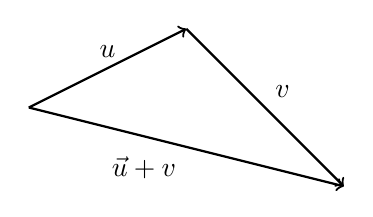
\begin{tikzpicture}
	\draw[->, thick] (-1,1) -- node[above] {$\vect{\mat{u}}$} (1,2);
	\draw[->, thick] (1, 2) --node[above right] {$\vect{\mat{v}}$}  (3, 0);
	\draw[->,thick] (-1, 1) -- node[below left] {$ \vec{\mat{u}} + \vect{\mat{v}}$} (3, 0);
	\end{tikzpicture}
\caption{Illustration de l'inégalité du triangle dans le plan cartésien: la somme des longueurs de deux 
des côtés d'un triangle est plus grande que la longueur du troisième côté.}
\end{marginfigure}
\noindent et donc $\norm{\mat{u} + \mat{v}}^2 \leq  \left( \norm{\mat{u}} + \norm{\mat{v}} \right)^2$.
En prenant la racine carrée de chaque côté, on obtient le résultat recherché.

\begin{exerciceB}
Démontrez l'inégalité triangulaire pour les vecteurs complexes. 
Vous voudrez possiblement utiliser le fait que, pour un nombre complexe de la
forme $a+bi$, nous avons
\[
a+bi + \overline{a+bi} = 2a \leq \sqrt{a^2 + b^2} = \abs{a+bi}
\]
\end{exerciceB}

\subsection{Exemples}
Pour chaque espace vectoriel, on peut définir un produit scalaire.  En voici quelques exemples.
\begin{enumerate}
\item Soit $V$ l'espace des matrices $m\times n$ sur $\BBR$. On peut définir un produit
scalaire de la façon suivante:
\[
\langle \matA, \matB \rangle = \tr(\transp{\matB}\matA)
\]
On note qu'en raison des propriétés de la multiplication des matrices, 
\[
(a\transp{\matA} + b\transp{\matB}) \matC = a\transp{\matA}\matC + b\transp{\matB}\matC
\]
l'axiome 1 de la définition d'un produit scalaire est automatiquement satisfait.
\item Soit $V$ l'espace des matrices $m\times n$ sur $\BBC$. On peut définir un produit
scalaire de la façon suivante:
\[
\langle \matA, \matB \rangle = \tr(\matB^*\matA)
\]
\item Soit $V$ l'espace des fonctions continues réelles sur l'intervalle $a\leq x \leq b$.
On peut définir un produit scalaire de la façon suivante:
\[
\langle f, g \rangle = \int_a^b f(x) g(x) dx
\]
\end{enumerate}

\begin{exerciceB}
Considérez des matrices générales réelles de taille $3\times 2$:
\[
\matA = \begin{pmatrix}
a_{11} & a_{12} \\
a_{21} & a_{22} \\
a_{31} & a_{32}
\end{pmatrix}
\qquad \mbox{et}\qquad\matB = \begin{pmatrix}
b_{11} & b_{12} \\
b_{21} & b_{22} \\
b_{31} & b_{32}
\end{pmatrix}
\]
Démontrez qu'en général $\transp{\matB}\matA \neq \transp{\matA}\matB$ mais que, néanmoins,
les axiomes 2, 3 et 4 de la définition d'un produit scalaire sont satisfait si on a
\[
\langle \matA, \matB \rangle = \tr(\transp{\matB}\matA)
\]
\end{exerciceB}

\begin{exerciceB}
Calculez la norme des matrices  $\displaystyle \begin{pmatrix}
0 & 1 \\
4 & 8
\end{pmatrix}$ et $\displaystyle \begin{pmatrix}
4 & -1 \\
-4 & 4
\end{pmatrix}$ en utilisant la définition mentionnée ci-dessus pour le produit scalaire
de matrices.
\end{exerciceB}

Un cas particulier du premier exemple est celui des matrices $m\times 1$ c'est-à-dire les
vecteurs de $\BBR^n$. Par exemple, pour $\BBR^3$, on peut avoir:
\[
\matX = \begin{pmatrix}
x_1 \\ x_2 \\ x_3
\end{pmatrix} \qquad\mbox{et}\qquad \matY= \begin{pmatrix}
y_1 \\ y_2 \\ y_3
\end{pmatrix}
\]
et donc
\[
\langle\matX, \matY\rangle = \tr(\transp{\matY}\matX) = \tr\left[ 
\begin{pmatrix}
y_1 & y_2 & y_3
\end{pmatrix}
\begin{pmatrix}
x_1 \\ x_2 \\ x_3
\end{pmatrix} \right]
= \tr(y_1 x_1 + y_2 x_2 + y_3 x_3) = y_1 x_1 + y_2 x_2 + y_3 x_3
\]
Habituellement, \textbf{par convention} pour les vecteurs de $\BBR^n$, 
au lieu d'utiliser la notation $\langle\matX, \matY\rangle$ on
écrira plutôt\footnote{En raison du point qui est utilisé entre les vecteurs
pour indiquer la multiplication scalaire, on appelle ceci \textit{\textbf{dot} product} en 
anglais. Le produit scalaire général est habituellement appelé \textit{inner product} 
en anglais.} $\matX\cdot\matY = \langle\matY, \matX\rangle$ 
et on traitera une matrice $1\times 1$ comme un
scalaire ce qui nous permettra d'omettre le symbole pour la trace. Ceci veut
dire qu'on écrira pour le produit dans $\BBR^3$
\[
\matX\cdot\matY = \begin{pmatrix}
x_1 & x_2 & x_3
\end{pmatrix}
\begin{pmatrix}
y_1 \\y_2 \\ y_3
\end{pmatrix} = x_1 y_1 + x_2 y_2 + x_3 y_3
\]
On peut facilement vérifier que $\matX\cdot\matY = \matY\cdot\matX$, que $\matX\cdot\matX\geq 0$ et que $\matX\cdot\matX = 0$ si et seulement si $\matX=\zero$.
\section{Orthogonalité}
\begin{defini}
Deux vecteurs $\mat{u}$ et $\mat{v}$ sont dits orthogonaux si $\langle \mat{u}, \mat{v}\rangle = 0$.
\end{defini}

Une base formée de vecteurs orthogonaux est appelée une \definition{base orthogonale}.

\begin{exerciceB}\label{ex:orthogonal}
Vérifiez que les matrices suivantes sont orthogonales:
\[
\begin{pmatrix}
1 & 0 \\ 0 & 0
\end{pmatrix}\qquad
\begin{pmatrix}
0 & 1 \\ 0 & 0
\end{pmatrix}\qquad
\begin{pmatrix}
0 & 0 \\ 1 & 0
\end{pmatrix}\qquad
\begin{pmatrix}
0 & 0 \\ 0 & 1
\end{pmatrix}
\]
\end{exerciceB}

\begin{theo}
\Definition{Théorème de Pythagore:} Deux vecteurs réels, $\mat{u}$ et $\mat{v}$, sont orthogonaux si et seulement si :
\[
\norm{\mat{u}+\mat{v}}^2 = \norm{\mat{u}}^2 + \norm{\mat{v}}^2
\] 
\vspace{-20pt}
\proof
Si on a deux vecteurs réels, alors $\langle \mat{u}, \mat{v}\rangle = \langle \mat{v}, \mat{u}\rangle$ et
\[
\begin{matrix}[rcl]
\norm{\mat{u} + \mat{v}}^2 &=& \langle \mat{u} +\mat{v},\mat{u} + \mat{v} \rangle \\
&=& \langle \mat{u}, \mat{u} \rangle + \langle \mat{u}, \mat{v} \rangle + \langle \mat{v}, \mat{u} \rangle + \langle \mat{v}, \mat{v} \rangle\\
&=& \norm{\mat{u}}^2 + 2\langle \mat{u}, \mat{v} \rangle  + \norm{\mat{v}}^2 
\end{matrix}
\]
d'où l'on obtient $\norm{\mat{u}+\mat{v}}^2 - \norm{\mat{u}}^2 - \norm{\mat{v}}^2 = 2\langle \mat{u}, \mat{v} \rangle$. Si les deux vecteurs sont
orthogonaux, le côté droit de l'égalité est zéro et le théorème de Pythagore est satisfait.  Si le théorème de Pythagore est
satisfait, alors le côté gauche de l'égalité est zéro, ce qui signifie que le produit scalaire des deux vecteurs est égal à zéro et donc
qu'ils sont orthogonaux.
\end{theo}

Le concept d'\definition{orthogonalité} est relié à celui d'\definition{indépendance linéaire}; en fait, on pourrait dire qu'il s'agit d'un cas extrême d'indépendance
linéaire.  
Supposons que l'on ait deux vecteurs orthogonaux non nuls,  $\mat{u}$ et $\mat{v}$, 
et que l'on essaie de trouver deux constantes,
$\alpha$ et $\beta$ telles que
\[
\alpha\mat{u} + \beta\mat{v} = \zero
\]
En prenant le produit scalaire de cette équation avec $\mat{u}$ on trouve $\alpha \norm{\mat{u}}^2 = 0$ ce qui implique que $\alpha=0$.
En prenant le produit scalaire de cette équation avec $\mat{v}$, on trouve que $\beta = 0$.  Donc, la seule façon que l'on puisse avoir
\[
\alpha\mat{u} + \beta\mat{v} = \zero
\]
est si les deux constantes, $\alpha$ et $\beta$ sont zéros.  
Par la définition de la dépendance linéaire, ceci veut dire que les vecteurs $\mat{u}$ et 
$\mat{v}$ sont linéairement indépendants.  Par contre l'inverse n'est pas vrai: deux
vecteurs linéairement indépendants ne sont pas nécessairement orthogonaux.  Par contre,
étant donné un ensemble de vecteurs linéairement indépendants, on peut obtenir un ensemble
de vecteurs orthogonaux. 
Supposons que l'on a deux vecteurs linéairement indépendants, $\mat{u}$ et $\mat{v}$.
Écrivons le vecteur $\mat{w}$ comme la combinaison linéaire suivante:
\[
\mat{w} = \mat{v} + \alpha\mat{u}
\]
et choisissons $\alpha$ tel que $\mat{w}$ et $\mat{u}$ soit orthogonaux:
\[
0 = \langle \mat{w}, \mat{u} \rangle = \langle (\mat{v} + \alpha\mat{u}), \mat{u}\rangle =
\langle\mat{v}, \mat{u}\rangle + \alpha \langle \mat{u}, \mat{u}\rangle
\]
\[
\Rightarrow \alpha = - \frac{\langle\mat{v}, \mat{u}\rangle}{\norm{\mat{u}}^2}
\]
On peut vérifier que $\Vect(\{\mat{u}, \mat{w}\}) = \Vect(\{\mat{u}, \mat{v}\})$.

On peut généraliser ceci à la situation où on a $n$ vecteurs linéairement indépendants.
Soit un tel ensemble $\{\mat{v}_1, \ldots \mat{v}_n \}$.
Choisissons $\mat{u}_1 = \mat{v}_1$.  Puis
\[
\mat{u}_2 = \mat{v}_2 - \frac{\langle\mat{v}_2, \mat{u}_1\rangle}{\norm{\mat{u}_1}^2}\mat{u}_1
\]
On peut vérifier que
\[
\langle\mat{u}_2, \mat{u}_1\rangle = \langle\mat{v}_2, \mat{u}_1\rangle  - \frac{\langle\mat{v}_2, \mat{u}_1\rangle}{\norm{\mat{u}_1}^2}\langle\mat{u}_1, \mat{u}_1\rangle = 0
\]
On peut continuer avec le troisième vecteur:
\[
\mat{u}_3 = \mat{v}_3 - \left(\frac{\langle\mat{v}_3, \mat{u}_1\rangle}{\norm{\mat{u}_1}^2}\mat{u}_1
+ \frac{\langle\mat{v}_3, \mat{u}_2\rangle}{\norm{\mat{u}_2}^2}\mat{u}_2\right)
\]
ou, de façon générale, le $n^{ième}$ vecteur
\[
\mat{u}_n = \mat{v}_n - \left(\frac{\langle\mat{v}_n, \mat{u}_1\rangle}{\norm{\mat{u}_1}^2}\mat{u}_1 + \ldots  
+ \frac{\langle\mat{v}_n, \mat{u}_{n-1}\rangle}{\norm{\mat{u}_{n-1}}^2}\mat{u}_{n-1}\right)
\]
de telle sorte que $\{\mat{u}_j\}$ sera un ensemble orthogonal et que
$\Vect(\{\mat{u}_j\}) = \Vect(\{\mat{v}_j\})$. La méthode que nous venons d'utiliser pour
obtenir un ensemble de vecteurs orthogonaux à partir d'un ensemble de vecteurs
linéairement indépendants est connue sous le nom de 
\definition{procédé d'orthogonalisation de Gram-Schmidt}. Voyons-en un exemple concret.

\begin{exemple}\label{ex:orthog}
Soient une base de $\BBR^3$ formée par l'ensemble des vecteurs
\[
\left\{ \mat{u}_1,\mat{u}_2,\mat{u}_3 \right\} =
\left\{ \begin{pmatrix}
1 \\ 1 \\ 0
\end{pmatrix} ,  \begin{pmatrix}
0 \\ 1 \\ 1
\end{pmatrix},  \begin{pmatrix}
1 \\ 0 \\ 1
\end{pmatrix}
\right\}
\]
À partir de cette base, obtenez un autre base contenant le vecteur $\mat{u}_1$ et
uniquement des vecteurs orthogonaux. 
\solution
Nous utilisons la procédure de Gram-Schmidt.  Nous avons:
\[
\mat{v}_1 = \mat{u}_1
\]
\[
\mat{v}_2 = \mat{u}_2 - \frac{\langle\mat{u}_2, \mat{v}_1\rangle}{\norm{\mat{v}_1}^2}\mat{v}_1
\] 
avec
\[
\norm{\mat{v}_1}^2 = \tr\left(\begin{pmatrix}
1 & 1 & 0
\end{pmatrix}\begin{pmatrix}
1 \\ 1 \\ 0
\end{pmatrix}\right) = 2
\]
et
\[
\langle\mat{u}_2, \mat{v}_1\rangle = \tr\left(\begin{pmatrix}
1 & 1 & 0
\end{pmatrix}\begin{pmatrix}
0 \\ 1 \\ 1
\end{pmatrix}\right) = 1
\]
de telle sorte que
\[
\mat{v}_2 = \begin{pmatrix}
0 \\ 1 \\ 1
\end{pmatrix} - \frac12 \begin{pmatrix}
1 \\ 1 \\ 0
\end{pmatrix} =
 \begin{pmatrix}
-\frac12 \\[7pt] \frac12 \\[7pt] 1
\end{pmatrix}
\]
\pagebreak
Le troisième vecteur est obtenu de façon semblable
\[
\mat{v}_3 = \mat{u}_3 - \frac{\langle\mat{u}_3, \mat{v}_1\rangle}{\norm{\mat{v}_1}^2}\mat{v}_1
- \frac{\langle\mat{u}_3, \mat{v}_2\rangle}{\norm{\mat{v}_2}^2}\mat{v}_2
\] 
avec
\[
\norm{\mat{v}_2}^2 = \tr\left(\begin{pmatrix}
-\frac12 & \frac12 & 1
\end{pmatrix}\begin{pmatrix}
-\frac12 \\[7pt] \frac12 \\[7pt] 1
\end{pmatrix}\right) = \frac32
\]
\[
\langle\mat{u}_3, \mat{v}_1\rangle = \tr\left(\begin{pmatrix}
1 & 1 & 0
\end{pmatrix}\begin{pmatrix}
1 \\ 0 \\ 1
\end{pmatrix}\right) = 1
\]
et
\[
\langle\mat{u}_3, \mat{v}_2\rangle = \tr\left(\begin{pmatrix}
-\frac12 & \frac12 & 1
\end{pmatrix}\begin{pmatrix}
1 \\ 0 \\ 1
\end{pmatrix}\right) = \frac12
\]
ce qui nous donne
\[
\mat{v}_3 = \begin{pmatrix}
1 \\ 0 \\ 1
\end{pmatrix}
- \frac12 \begin{pmatrix}
1 \\ 1 \\ 0
\end{pmatrix}
- \frac13 \begin{pmatrix}
-\frac12 \\[7pt] \frac12 \\[7pt] 1
\end{pmatrix}
= \begin{pmatrix}
\frac23 \\[7pt] -\frac23 \\[7pt] \frac23
\end{pmatrix}
\]
La base recherchée est donc
\[
\left\{   \begin{pmatrix}
1 \\ 1 \\ 0
\end{pmatrix}, 
 \begin{pmatrix}
-\frac12 \\[7pt] \frac12 \\[7pt] 1
\end{pmatrix}, 
 \begin{pmatrix}
\frac23 \\[7pt] -\frac23 \\[7pt] \frac23
\end{pmatrix} \right\}
\]
\end{exemple}

\begin{exerciceB}\label{prob:orthog}
Soit la base suivante pour les matrices symétrique $2\times 2$
\[
\left\{\mat{u}_1, \mat{u}_2, \mat{u}_3 \right\} = \left\{ \begin{pmatrix}
2 & 0 \\
0 & 0
\end{pmatrix},
\begin{pmatrix}
1 & 1\\ 1 & 0
\end{pmatrix},
\begin{pmatrix}
0 & 1 \\
1 & 2
\end{pmatrix}
\right\}
\]
À partir de cette base, obtenez un autre base contenant le vecteur\footnote{J'utilise ici
le mot vecteur dans le sens général d'élément d'un espace vectoriel; 
il s'agit bel et bien d'une matrice.  La raison pour laquelle je mentionne
ceci est qu'il existe un type de matrice qu'on appelle une matrice orthogonale
et qui n'a rien à voir avec le produit scalaire. On dit d'une matrice $\matA$
qu'elle est orthogonale si elle obéit l'équation $\transp{\matA}=\matA^{-1}$.} $\mat{u}_1$ et
uniquement des vecteurs orthogonaux en utilisant la procédure de Gram-Schmidt.
\end{exerciceB}
\begin{exerciceB}
Utilisez la méthode habituelle (matrice augmentée, élimination de Gauss-Jordan, etc.) 
pour exprimer la matrice symétrique 
\[
\matA = \begin{pmatrix}
1 & 4 \\ 4 & 3
\end{pmatrix}
\]
comme une combinaison linéaire des trois vecteur orthogonaux (matrices de la base) trouvés à
l'\refexercice{prob:orthog}.
 Vérifiez que la combinaison linéaire que vous avez trouvée est
effectivement égale à la matrice ci-dessus.
\end{exerciceB}

\begin{defini}
Un ensemble de vecteurs $\mat{v}_j$ est dit \index{orthonormé}\textbf{orthonormé} 
si tous les vecteurs
sont orthogonaux et que la norme de chaque vecteur est égale à 1
\[
\langle \mat{v}_i, \mat{v}_j \rangle = \delta_{ij} = \left\{
\begin{matrix}
0 \, \mbox{si} \, i \neq j \\
1 \, \mbox{si} \, i = j
\end{matrix}\right.
\]
Une base formée de tels vecteurs est appelée soit 
\index{base orthonormée}\textbf{base orthonormée} ou
\index{base orthonormale}\textbf{base orthonormale}.
\end{defini}
\begin{exemple}\label{ex:orthon}
À partir de la base orthogonale trouvée dans l'\refexemple{ex:orthog}, obtenez une base orthonormée.
\solution
Il suffit de diviser chacun des vecteurs par sa norme.
$\displaystyle \mat{w}_j = \frac{\mat{v}_j}{\norm{\mat{v}_j}}  $\\
On peut vérifier que
$\norm{\mat{v}_1} = \sqrt{2}, \norm{\mat{v}_2}=\sqrt{\frac32}, \norm{\mat{v}_3}=\sqrt{\frac43}$
ce qui nous permet d'écrire la base orthonormée de la façon suivante:
\[
\{\mat{w}_1, \mat{w}_2, \mat{w}_3\} = \left\{
\frac{\sqrt{2}}{2}\begin{pmatrix}
1 \\ 1 \\ 0
\end{pmatrix},
\frac{\sqrt{6}}{6}
\begin{pmatrix}
-1 \\ 1 \\ 2
\end{pmatrix},
\frac{\sqrt{3}}{3}
\begin{pmatrix}
1 \\ -1 \\ 1
\end{pmatrix}
\right\}
\]
\end{exemple}

\begin{exerciceB}
Vérifiez que la norme de chacune des matrices de l'\refexercice{ex:orthogonal} est 1, et
donc que ces matrices forment un ensemble orthonormé.
\end{exerciceB}

\begin{exerciceB} \label{prob:orthog2}
À partir de la base orthogonale trouvée dans l'\refexercice{prob:orthog}, obtenez une base orthonormée.
\end{exerciceB}

Le grand avantage des bases orthonormées est qu'elles nous permettent de trouver rapidement
décomposition d'un vecteur quelconque dans cette base.  Par exemple, supposons que
la base $\{\mat{w}_1, \mat{w}_2, \mat{w}_3\}$  et que l'on veuille écrire un vecteur
quelconque $\mat{v}$ comme une combinaison linéaire des trois vecteurs de cette base:
\[
\mat{v} = \alpha_1\mat{w}_1 + \alpha_2\mat{w}_2 + \alpha_3\mat{w}_3
\]
Pour trouvez les trois inconnues, $\alpha_j$, il suffit de prendre le produit scalaire
avec le vecteur $\mat{w}_j$; par exemple:
\begin{eqnarray*}
\langle \mat{v}, \mat{w}_1\rangle &=&
 \alpha_1\color{blue}
 \underbrace{\color{black}\langle\mat{w}_1, \mat{w}_1\rangle}_1\color{black} +
 \alpha_2\color{blue}\underbrace{\color{black}\langle\mat{w}_1, \mat{w}_2\rangle}_0
  \color{black}+ \alpha_3\color{blue}\underbrace{\color{black}\langle\mat{w}_1,
   \mat{w}_3\rangle}_0 \\
 &=& \alpha_1
\end{eqnarray*}
 puisque $\langle\mat{w}_1, \mat{w}_j\rangle = \delta_{1j}$.  Nous n'avons donc pas 
 de système d'équations linéaires à résoudre!

\begin{exemple}
Exprimez le vecteur $\mat{v} = \transp{(x,y,z)}$ comme une combinaison linéaire des vecteurs
de la base orthonormée de l'\refexemple{ex:orthon}.
\solution
Nous avons
\[
\langle\mat{v}, \mat{w}_1\rangle = \tr\left(
\frac{\sqrt{2}}{2}\begin{pmatrix}
1 & 1 & 0
\end{pmatrix}\begin{pmatrix}
x \\ y \\ z
\end{pmatrix}\right) = \frac{\sqrt{2}}{2}(x+y)
\]
\[
\langle\mat{v}, \mat{w}_2\rangle = \tr\left(
\frac{\sqrt{6}}{6}
\begin{pmatrix}
-1 & 1 & 2
\end{pmatrix}\begin{pmatrix}
x \\ y \\ z
\end{pmatrix}\right) = \frac{\sqrt{6}}{6}(-x+y+2z)
\]
et
\[
\langle\mat{v}, \mat{w}_2\rangle = \tr\left(
\frac{\sqrt{3}}{3}
\begin{pmatrix}
1 & -1 & 1
\end{pmatrix}\begin{pmatrix}
x \\ y \\ z
\end{pmatrix}\right) = \frac{\sqrt{3}}{3}(x-y+z)
\]
ce qui nous permet d'écrire
\[
\begin{pmatrix}
x\\y\\z
\end{pmatrix}= \frac{x+y}{2} \begin{pmatrix}
1 \\ 1 \\ 0
\end{pmatrix}
+ \frac{-x+y+2z}{6} \begin{pmatrix}
-1 \\ 1 \\ 2
\end{pmatrix}
+ \frac{x-y+z}{3}\begin{pmatrix}
1 \\ -1 \\ 1
\end{pmatrix}
\]
\end{exemple}
\begin{exerciceB}
Utilisez les produits scalaires 
pour exprimer la matrice symétrique 
\[
\matA = \begin{pmatrix}
1 & 4 \\ 4 & 3
\end{pmatrix}
\]
comme une combinaison linéaire des trois vecteurs orthonormées (matrices de la base) trouvés à
l'\refexercice{prob:orthog2}. Vérifiez que la combinaison linéaire que vous avez trouvée est
effectivement égale à la matrice ci-dessus.
\end{exerciceB}


